\chapter{Results and Analysis}
\label{Chapter:Results}

\section{Serpent Model}
The actuator characterization methodology described in Section \ref{Section:Serpent} is extensive and computationally expensive. Before conducting the main study, some simpler codes were run to ensure that these efforts were spent on a viable design. The reactor must have adequate excess reactivity to overcome equilibrium poisoning and several years of depletion. Conversely, adequate shut-down margin is required to ensure that the reactor can be scrammed even in the event of a partial failure to the control drum drives. Finally, as the \acs{msnb} is meant to operate for extended periods of time without significant maintenance, the control material should still be effective at the end of the reactor lifetime. With the results of these three simple studies in mind, the neutron spectra in key regions of the \acs{msnb} are investigated to recommend improvements to the design that may warrant future work.

\subsection{Excess Reactivity and Shut-down Margin}
Excess reactivity is calculated by orienting the \acs{msnb} in its most reactive control position with fresh fuel and running a criticality model. The neutron multiplication factor (k\textsubscript{eff}) predicted by Serpent is converted to reactivity, and the magnitude above zero is reported as the excess reactivity of the design: 

\begin{equation}
    \rho = \frac{k_{eff}-1}{k_{eff}}
\end{equation}

After several iterations, the design used in this work was found to have an excess reactivity of 4.834\% $\pm$ 45.3 pcm with an average core temperature of 650 \textsuperscript{o}C. This is generally considered to be a slim margin, although the relatively low specific power reduces the equilibrium poison levels and the rate of fissile depletion, and aligns with previous work conducted on a similar design \cite{PetersonMS}. In this work, the initial batch of fuel lasted nearly 6 years before the total loss of excess reactivity was observed.

\begin{figure}[!ht]
    \centering
    \subfloat[\centering Single Misfire]{\includegraphics[width=0.48\textwidth]{Plotter/0.0shutdown7drum/MSNB_geom4}}
    \subfloat[\centering Single Success]{\includegraphics[width=0.48\textwidth]{Plotter/0.0shutdown1drum/MSNB_geom4}}
    \caption[X-Y View of \acs{msnb} - Shut-Down Margin]{X-Y Views of \acs{msnb} with control drums in two shut-down margin failure modes:
    \begin{enumerate*}[label=\alph*)]
        \item Seven drums in least reactive orientation, one drum failed in most reactive orientation; and 
        \item One drum in least reactive orientation, seven drums failed in most reactive orientation; 
    \end{enumerate*}
    The entire wedge of each control drum is colored for clarity. Only the outer rim is actually made from boron carbide.}
    \label{fig:Plotter-SDM}
\end{figure}

The shut-down margin is found using a similar methodology, placing the \acs{msnb} in a very low reactivity orientation and observing the results of the criticality model. With all 8 control drums facing inward, this design has a 54.76\% $\pm$ 103 pcm shut-down margin. This is an extremely high shut-down margin, meaning that only a fraction of the reactor's available control reactivity is needed to carry-out an emergency shut-down. 

\acsp{lwr} are required to maintain 1\% shut-down margin with the most reactive control rod failing to actuate \cite{Margin}. Two further case studies were conducted, as depicted by Figure \ref{fig:Plotter-SDM}, to study the effect of actuation failures. First, a shut-down margin of 47.19\% $\pm$ 91.0 pcm was calculated for the \acs{msnb} in the event that one of the control drums sticks in its most reactive orientation. Then, a worst case scenario, where only one control drum successfully actuates was found to have a shut-down margin of 0.417\% $\pm$ 46.4 pcm with fresh, un-poisoned fuel. It is extremely unlikely that 7 out of 8 drums would fail to actuate in an emergency, assuming a well designed fail-safe and redundant system. Even in this unlikely event, the \acs{msnb} could be safely shut-down.

\subsection{Control Material Longevity}
Boron carbide was selected as the control material for this design because it simultaneously provided adequate shut-down margin and excess reactivity. It is, however, a burnable neutron poison, meaning that a \B[10] atom can only absorb one neutron. In the interest of keeping maintenance to the \acs{msnb} to a minimum, the control drums cannot lose their ability to insert control reactivity during the expected life of the reactor. The control material was burned at full power (10 MWth) for ten years, and the change to the concentrations of key nuclides were plotted in Figure \ref{fig:BoronBurn}.

\begin{figure}[ht!]
    \centering
    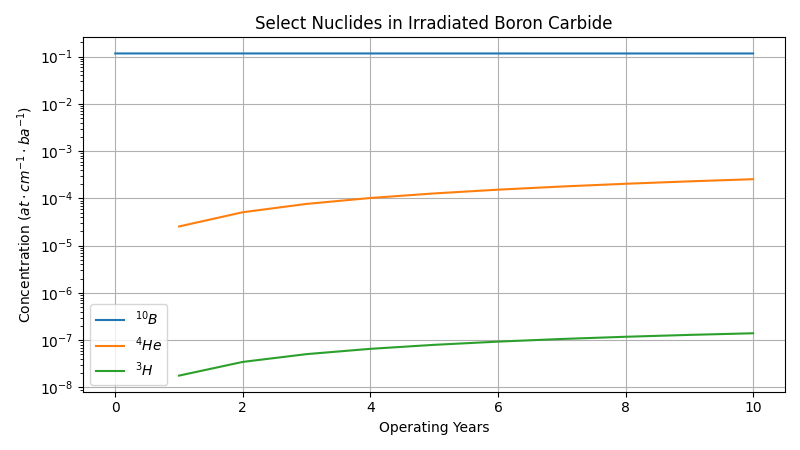
\includegraphics[width=0.9\textwidth]{./Plotter/boronburn/AtomDens}
    \caption[\acs{msnb} Irradiated Boron Carbide]{Concentration of tritium, helium-4, and boron-10 in irradiated boron carbide during a decade-long \acs{msnb} deployment.}
    \label{fig:BoronBurn}
\end{figure}

After 100 MW-yr of heat output, just 0.22\% of the \B[10] was consumed. This caused a negligible effect on the reactivity worth of each control drum. In addition to the deactivation of the neutron poison itself, two gases of interest are formed in boron carbide under neutron fluence. Helium-4 is formed after the alpha particle from the primary capture reaction is de-ionized:

\begin{reaction} \label{rxn:B10cap}
    ^{10}B + n \to {^{7}Li} + \alpha
\end{reaction}

By the end of the decade scale operation, 58 moles of helium have been formed by this pathway. This is a significant amount that will need to be off-gassed operation, and could cause swelling if the material is not properly qualified. Tritium is also formed both directly and indirectly by the $^{10}B(n,2\alpha){^{3}H}$ and $^{7}Li(n,n\alpha){^{3}H}$ reactions. At the end of the study, the control material of the \acs{msnb} contained 31.9 millimoles, or 95.7 mg of tritium. This will account for a small amount of the total radioactivity in the decommissioned \acs{msnb}.

\subsection{Neutron Spectra}


\begin{figure}[ht!]
    \centering
    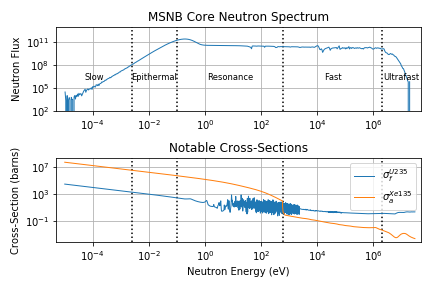
\includegraphics[width=0.9\textwidth]{./Plotter/Detector/Spectrum}
    \caption[\acs{msnb} Neutron Energy Spectrum]{\raggedright \acs{msnb} neutron energy spectrum in core, reflector, and downcomer.}
    \label{fig:Spectrum}
\end{figure}


\subsection{Actuator Curve}\label{sec:actuator}

\begin{figure}[!ht]
    \centering
    \subfloat[\centering Xenon-135 Build-up]{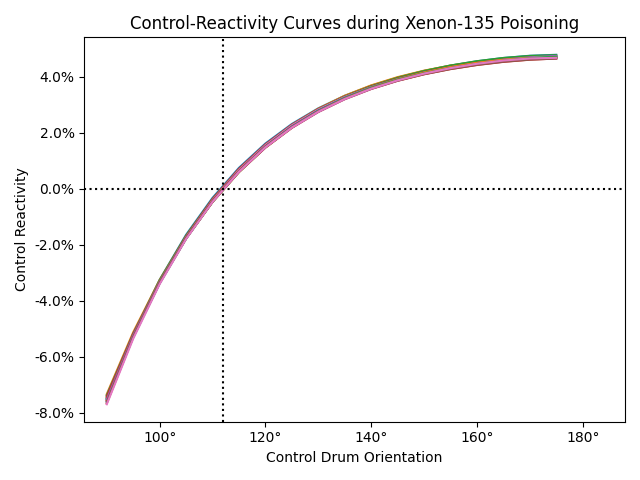
\includegraphics[width=0.49\textwidth]{/CurveFits/eqXe}}
    \subfloat[\centering Depletion]{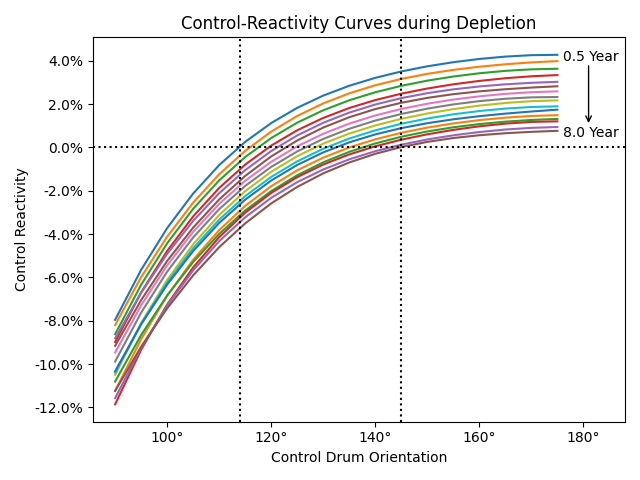
\includegraphics[width=0.49\textwidth]{/CurveFits/depletion}}
    \caption[Control Reactivity Curve]{Control drum angle vs. reactivity curves. Each curve corresponds to a different burn-up level:
    \begin{enumerate*}[label=\alph*)]
        \item 6 hour increments until \Xe reaches equilibrium`'; and 
        \item 6 month increments until the fuel is depleted enough that the \acs{msnb} has very little excess reactivity; 
    \end{enumerate*}
    }
    \label{fig:ControlReactivityCurve}
\end{figure}

\section{Multi-physics Simulation}

\subsection{Steady-State}

\subsection{Up-Step}
autonomous
controller tuning
controlled response


\subsection{Down-Step}

\subsection{Start-Up}

\subsection{Shut-Down}

\subsection{Demand-Response}